\documentclass[crop,convert={density=600,outext=.png}]{standalone}

\usepackage{tikz}
 
\begin{document}
 
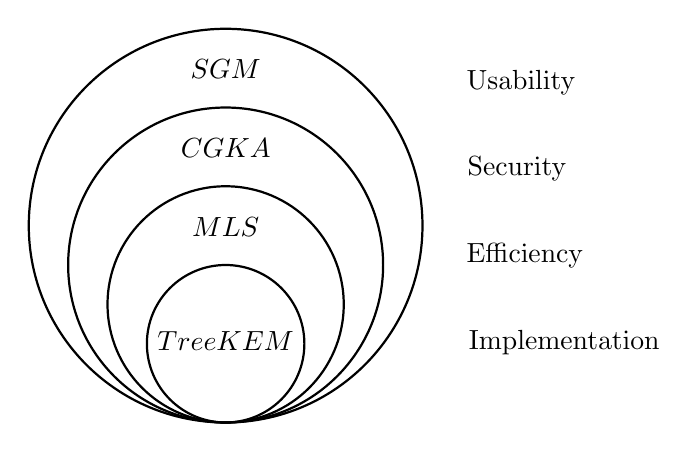
\begin{tikzpicture}[thick]
 
% Set A
\node[label={$SGM$}] (A) at (0,0.6) {};
 
% Set B
\node[label={$CGKA$}] (B) at (0,-0.4) {};
 
% Set C
\node[label=$MLS$] (C) at (0, -1.4) {};

% Set D
\node[label=$TreeKEM$] (D) at (0,-2.85) {};

\node[label={Usability}]      (W) at (3.75, 0.4) {};
\node[label={Security}]       (X) at (3.7,-0.7) {};
\node[label={Efficiency}]     (Y) at (3.8,-1.8) {};
\node[label={Implementation}] (Z) at (4.3,-2.9) {};


\draw (0,-1) circle(2.5cm);
\draw (0,-1.5) circle(2cm);
\draw (0,-2) circle(1.5cm);
\draw (0,-2.5) circle(1cm);
 
\end{tikzpicture}
 
\end{document}
